%% The layout here is based on the APS REVTeX 4 template, Version 4.1r of REVTeX, August 2010.

% Group addresses by affiliation; use superscriptaddress for long
% author lists, or if there are many overlapping affiliations.
% For Phys. Rev. appearance, change preprint to twocolumn.
% Choose pra, prb, prc, prd, pre, prl, prstab, prstper, or rmp for journal
%  Add 'draft' option to mark overfull boxes with black boxes
%  Add 'showpacs' option to make PACS codes appear
%  Add 'showkeys' option to make keywords appear

%latexdiff-so file1.tex file2.tex > diff.tex

\documentclass[reprint,amsmath,amssymb,aps,prl,groupedaddress,nofootinbib,superscriptaddress]{revtex4-1}
%\documentclass[aps,prl,preprint,superscriptaddress]{revtex4-1}
%\documentclass[aps,prl,reprint,groupedaddress]{revtex4-1}
\usepackage{graphicx}
\usepackage{amsthm,amssymb,amsmath,braket,mathdots}
\usepackage{bm}
\usepackage[hidelinks,pagebackref=false,pdfnewwindow=true]{hyperref} %\hypersetup{draft}
%\usepackage{doi}
\usepackage{epstopdf,psfrag}
\usepackage{relsize,amsbsy}
\usepackage[export]{adjustbox}

\usepackage{graphicx,xcolor,tikz}


\DeclareMathOperator{\sgn}{sgn}
\DeclareMathOperator{\tr}{Tr}
\DeclareMathOperator{\re}{Re}
\DeclareMathOperator{\im}{Im}

\newcommand{\dd}{\partial}
\newcommand{\1}{\mathds{1}}

\newcommand{\mac}{\mathcal}
\newcommand{\be}{\begin{equation}}
\newcommand{\ee}{\end{equation}}

%\newcommand{\dd}{\partial}
%\newcommand{\1}{\mathds{1}}
\newcommand{\ms}{Majorana spinon }
\newcommand{\mss}{Majorana spinons }
\newcommand{\mssns}{Majorana spinons}
\newcommand{\hh}{harmonic honeycomb }
\newcommand{\HH}{Harmonic Honeycomb }
\newcommand{\Hs}[1]{\mbox{$\mathcal{H}$-$#1$}}

\newcommand{\bit}{\begin{enumerate}}
	\newcommand{\eit}{\end{enumerate}}
\newcommand{\m}{\item}
\newcommand{\zt}{\mathbb{Z}_2}
\def\em{\it}
\definecolor{bananayellow}{rgb}{1.0, 0.88, 0.21}
\definecolor{straw}{rgb}{0.32, 0.28, 0.1}

\newcommand{\fb}{\it \color{orange}}
\definecolor{palatinatepurple}{rgb}{0.49, 0.24, 0.46}
\newcommand{\bp}{ \color{straw} }
\definecolor{darkgreen}{rgb}{0.0, 0.5, 0.0}
\newcommand{\jk}{\it \color{darkgreen}}

\graphicspath{{Figures/}}

\begin{document}
	
	
	
	\title{Majorana Landau Level Spectroscopy  --  a proposal for observing pseudo magnetic fields in  strained thin films of $\alpha$-RuCl$_3$}
		\author{us}
%		\affiliation{\small School of Physics and Astronomy, University of Minnesota, Minneapolis, Minnesota 55455, USA}
%		%	\email[]{perre035@umn.edu}
%		%	%\homepage[]{https://www.physics.umn.edu/people/perreault.html}
%		%	
%		\author{Johannes Knolle}
%		\affiliation{\small Department of Physics, Cavendish Laboratory, JJ Thomson Avenue, Cambridge CB3 0HE, U.K.}
%		%	
%		\author{F. J. Burnell}
%		\affiliation{\small School of Physics and Astronomy, University of Minnesota, Minneapolis, Minnesota 55455, USA}
		
		\date{\today} 
		
		
		\begin{abstract}
		 	abstract
		\end{abstract}
		
		
		% insert suggested PACS numbers in braces on next line
		%\pacs{}
		% insert suggested keywords - APS authors don't need to do this
		%\keywords{}
		
		%\maketitle must follow title, authors, abstract, \pacs, and \keywords
		\maketitle
		
		%	\tableofcontents
		
		
		%{\jk Johannes}
		%{\bp Brent} {\fb Fiona}
	
	%\tableofcontents
	
	\section{Introduction}
	
{\bp	TODO: Add some mention of why we choose $\beta = 10$. There is a paragraph on this in the ``Notes." }
	
Lattice strain can induce effective magnetic fields without actually breaking time reversal symmetry. An out of plane (along the $z$-axis) magnetic field can be induced by strain fields of the form $B=\beta \left[2 \partial_x u_{xy}-\partial_y (u_{xx}-u_{yy}) \right]$. Here, in addition to our numerical evaluations we try to obtain a more microscopic understanding of the influence of such a pseudo magnetic field on a Majorana fermion system and how the expected Landau level degeneracy is manifest in the Raman response function. 

Via minimal coupling of the vector potential we use the canonical momenta $\mathbf{\Pi}= \mathbf{p}-\frac{e}{c} \mathbf{A}$ and work in the Landau gauge $\mathbf{A}=B(0,x)$. We study the low energy behaviour of our Majorana fermion systems in the flux free low temperature sector by expanding the Majorana field operators $\hat \Psi = \left( \Psi_{A}(\mathbf{r}) \Psi_{B}(\mathbf{r}) \right)^T$ around the two Dirac points (labeled by $\nu=\pm 1$)
\begin{eqnarray}
H_{\nu} \approx i \int \text{d}^2 \mathbf{r} 
\hat \Psi^{\dagger}
\begin{pmatrix}
0 & \nu p_x- i(p_y- \nu B x) \\
- \nu p_x- i(p_y-\nu B x) & 0 
\end{pmatrix}
\hat \Psi \nonumber .
\end{eqnarray}
Note that $B$ has opposite sign at the two Dirac points leaving TRS intact, which however prevents the usual trick of combining the two Majorana cones into a single cone of complex fermions. Nevertheless, we can concentrate on only one of the cones because there is no coupling between the two.  


We introduce the ladder operator $a=\frac{l}{2\hbar} \left(\Pi_x-i \Pi_y \right)$ with $l^2=\frac{c\hbar}{e|B|}$. Then we expand the field operators in terms of the standard Landau Level wave functions $\Psi_{A} (\mathbf{r}) = \sum_{n,p} \Phi_{n-1,p} (\mathbf{r}) f_{A n p}$ and $\Psi_{B} (\mathbf{r}) = \sum_{n,p} \Phi_{n,p} (\mathbf{r}) f_{B n p}$ with Majorana operators $f_{A/B n p}$ obeying the Majorana commutation relations (but note the sign change of momenta from conjugation $\Psi_{B}^{\dagger} (\mathbf{r}) = \sum_{n,p} \Phi^*_{n,p} (\mathbf{r}) f_{B n -p}$). Using the ladder operator properties $a \Phi_n=\sqrt{n} \Phi_{n-1}$ and $a^{\dagger} \Phi_n=\sqrt{n+1} \Phi_{n+1}$ we obtain the Hamiltonain
\begin{eqnarray}
H_{+}  & \approx & 
\begin{pmatrix}
f_{An-p} & f_{B n -p} 
\end{pmatrix}
\begin{pmatrix}
0 & i \frac{2 \hbar}{l} \sqrt{n} \\
- i \frac{2 \hbar}{l} \sqrt{n} & 0 
\end{pmatrix}
\begin{pmatrix}
f_{A n p} \\ f_{B n p} 
\end{pmatrix}.
\end{eqnarray}
It is diagonalized by introducing  the complex fermions $a_{np}$ with $f_{Bnp}=a_{np}+a^{\dagger}_{n-p}$ and $f_{Anp}=i \left(a_{np}  -a_{n-p}^{\dagger}\right)$ such that
\begin{eqnarray}
H_{+}  & \approx & 
\sum_{np} E(n) \left[ a_{np}^{\dagger} a_{np} -\frac{1}{2}\right] 
\end{eqnarray}
with the energies $E(n)=4 \frac{\sqrt{2\hbar}}{l} \sqrt{n}$ obeying the well known $\propto\sqrt{n}$ scaling of Dirac fermions. 

Next, we look at the low energy behaviour of the Raman response $I(\omega)=\int_{-\infty}^{\infty} \text{d}t e^{i\omega t} \langle R(t) R(0)\rangle$. The main difference between the non-resonant and resonant Raman vertices is that the former couples both sublattices whereas the latter does not
\begin{eqnarray}
R_{\text{non-res}} & \propto & i \int \text{d}^2 \mathbf{r}  \Psi^{\dagger}_A(\mathbf{r})(t) \Psi_B(\mathbf{r}) \\ \nonumber
& \propto & \sum_{np} \left[ a_{n-p}(t) -a^{\dagger}_{np} (t) \right] \left[ a_{n-1 p} + a^{\dagger}_{n-1 -p} \right] \\ \nonumber
R_{\text{res}} & \propto & i \int \text{d}^2 \mathbf{r} \left[ \Psi^{\dagger}_A(\mathbf{r})(t) \Psi_B(\mathbf{r+\delta}) - \Psi^{\dagger}_A(\mathbf{r})(t) \Psi_B(\mathbf{r-\delta}) \right] \\ \nonumber
& \propto & \sum_{np} \sin \left(p \delta \right) \left[ a_{n-p}(t) -a^{\dagger}_{np} (t) \right] \left[ a_{n p} + a^{\dagger}_{n -p} \right] .
\end{eqnarray}
The form of both vertices is very similar but only the non-resonant vertex mixes states which differ by one LL index. From the time dependence $a_{np}(t)=a_{np} e^{-i t E(n)}$ and $a_{np} |0\rangle=0$ we can directly calculate the low energy Raman responses
\begin{eqnarray}
I_{\text{non-res}} & \propto &  \sum_{np} \delta\left[\omega - E(n)-E(n+1) \right] \\ \nonumber
I_{\text{res}} & \propto &  \sum_{np} \delta\left[\omega - 2E(n)  \right] .
\end{eqnarray}
In agreement with the numerical observation we find different scaling of the resonant and non-resonant intensities which originates from the sub-lattice selectivity of the vertices and the special structure of LL wave functions in Dirac systems which mix adjacent LL indices. 



\begin{figure*}
	\centering
	\begin{tikzpicture}
	\node{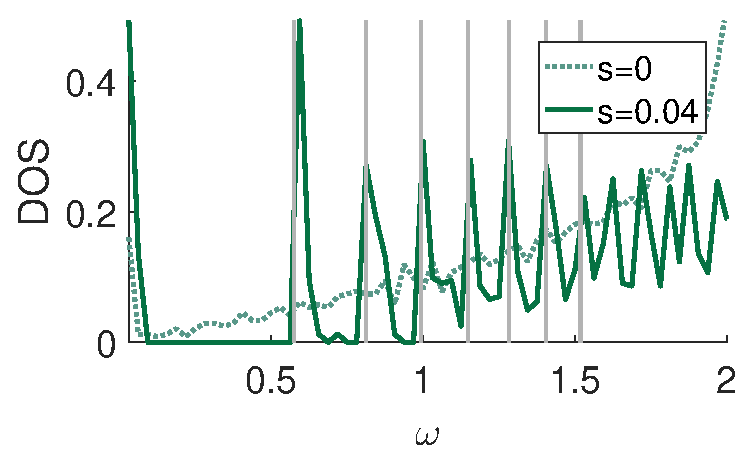
\includegraphics[width=0.32\linewidth]{stretch_DOS_special_rmax_50_b_10_c_40.eps}
		\quad
		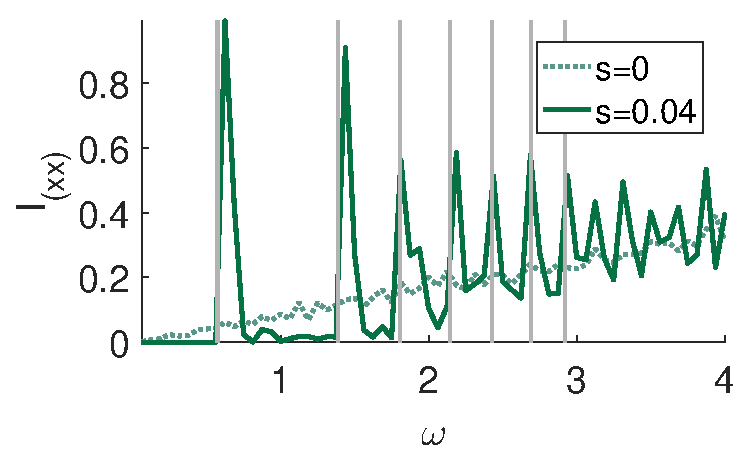
\includegraphics[width=0.32\linewidth]{stretch_I2_special_rmax_50_b_10_c_40.eps} 
		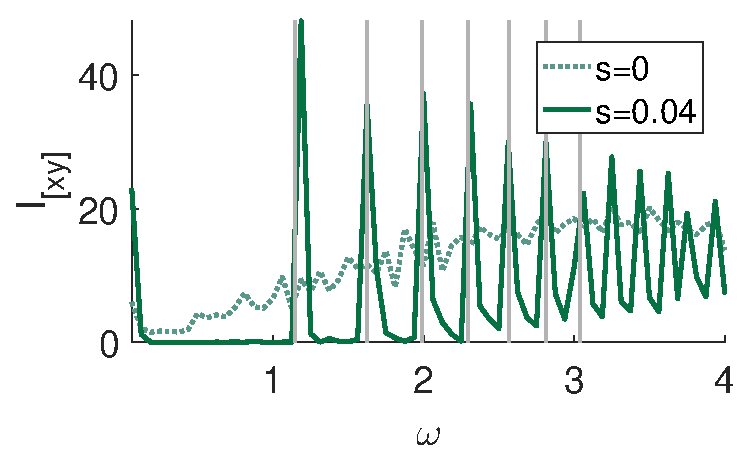
\includegraphics[width=0.32\linewidth]{stretch_I3_special_rmax_50_b_10_c_40.eps} } ;
	\node[] (image) at (-8.75,1.55) {(a)};
	\node[] (image) at (-2.70,1.55) {(b)};
	\node[] (image) at ( 3.35,1.55) {(c)};
	\end{tikzpicture}
	\caption{The DOS and all possible Raman correlation functions for $s=4$\% maximum strain and zero strain with $r=50$ corresponding to $6*(50+1)^2 = 15606$ sites. (a) shows peaks at $\sqrt{n}E_0$ while (b) has them at $(\sqrt{n} + \sqrt{n+1})E_0 $ and (c) $2 \sqrt{n} E_0$. One can see that the Landau level peaks are easily distinguishable from finite size effects at this system size and strain.}
	\label{basicPlots}
\end{figure*}

\begin{figure*}
	\centering
	\begin{tikzpicture}
	\node{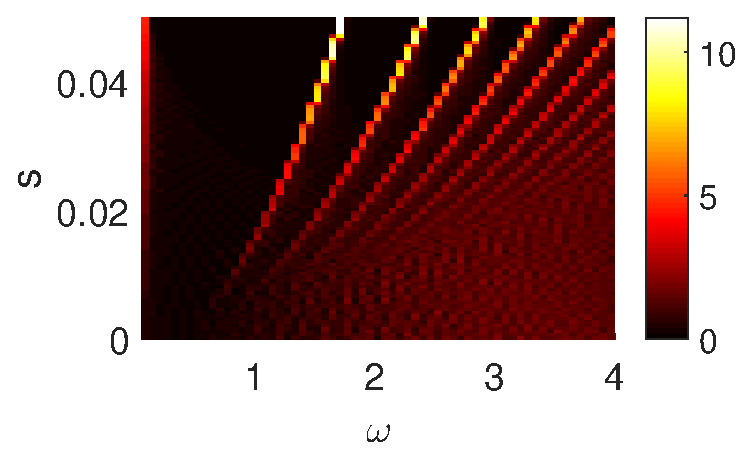
\includegraphics[width=0.32\linewidth]{stretch_comp_xy2_b_10_n_30_maxn_100_special.eps} 
		\quad
		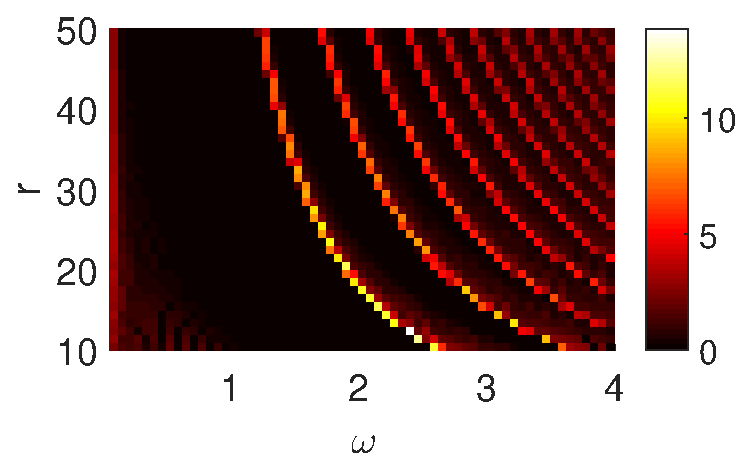
\includegraphics[width=0.32\linewidth]{size_comp_xy2_b_10_s_4_maxn_50_special.eps} 
		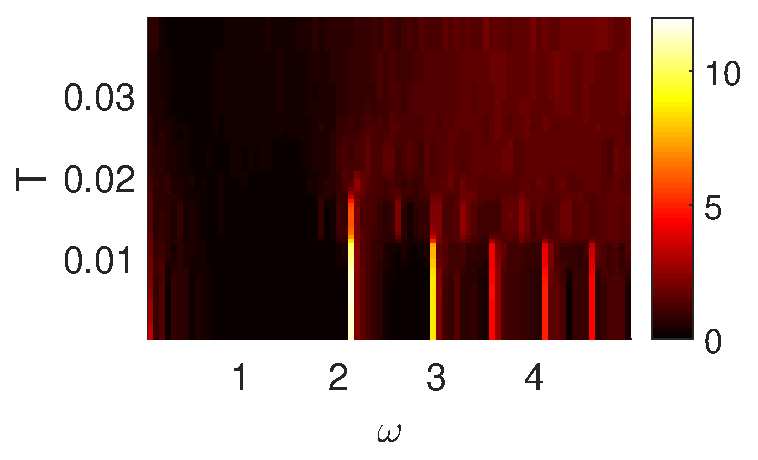
\includegraphics[width=0.32\linewidth]{stretch_comp_Ixy2_finiteT_b_rmax_15_b_10_s_40_special.eps}  } ;
	\node[] (image) at (-8.75,1.55) {(a)};
	\node[] (image) at (-2.75,1.55) {(b)};
	\node[] (image) at ( 3.25,1.55) {(c)};
	\end{tikzpicture}
	\caption{A set of density plots showing the progression of Landau level peaks as a function of (a) strain, (b) system size, and (c) temperature. Where not specified the strain is taken at $s=4$\% and $T=0$ with the system sizes (a) $r = 30$ and (c) $r = 15$. The temperature of the crossover in (c) agrees well with the expected spinon-confinement transition for non-interacting fluxes at $T_c \approx 0.02J$ for this system size, which is expected to be lowered slightly by flux-flux interactions.} 
	\label{colorPlots}
\end{figure*}

\section{Results} 
We follow the Refs.~\cite{Guinea10,Amal13,Rachel15} to study a honeycomb flake, strained in a way that preserves the $S_6$ lattice symmetry. With the strain pattern given by% to model a strained honeycomb flake. We take $x$ and $y$ to be the positions of a lattice site without any strain (the base configuration makes a perfect honeycomb), measured in units of $a_0$, the lattice constant (the distance between two NN sites). We then write
\begin{align}
\vec{u}(x,y) = C(2xy,x^2-y^2),
\end{align}
one obtains a uniform effective magnetic field with magnitude $B = -8 \beta C$. This pattern can be visualized as in Fig. \ref{honeycomb_flake} {\bp(Needs Figure)}.

We construct the honeycomb flake as $r$ layers of honeycombs placed around an initial single one as in Fig. \ref{honeycomb_flake} \cite{Rachel15}. We choose to characterize the strain by the total amount of strain along the directions of maximal stretching and compression $s = \frac{\delta L}{L} = \sqrt{3}C(r+\frac{1}{2})$ so that $B \approx \frac{4\beta}{\sqrt{3}r}s$. For linear elasticity to hold we need $s \ll \frac{\sqrt{3}}{2\beta}$. 

We take $\beta = 10$. For this case the optimal parameters are strains of $1$-$4$\% and system sizes of $r = 25$-$50$ unit cells. In RuCl$_3$ an unstrained honeycomb is about $6$\AA \ so that such flakes would have diameters of $30$-$60$nm. 
We find that for the magnetic field to be strong enough at to create noticeable Landau levels at these system sizes it needs to be on the order of $B\approx 0.03$ and that the levels appear/disappear sharply near that value. With increasing system size the maximum value of $B$ decays with $1/r$, putting constraints on how large the honeycomb flake can be. This is in competition with the need to have a large enough system to get a spectrum that is not too noisy. 

{\it Raman scattering.} 

Fig. \ref{basicPlots} and Fig. \ref{colorPlots} are awesome. blah blah blah. Something about how the temperature dependence makes the Landau levels a true signature of the deconfined spin liquid phase.

We used the notation $I_{[xy]}$ for the channel anti-symmetric in polarization. The subtraction required to isolate this channel was reviewed in Ref. \cite{Perreault16-1} (see supplemental). However, in practice one should see only the $\sqrt{n} + \sqrt{n+1}$ peaks in the channel $I_{xx}$, while near resonance the $I_{xy}$ channel should contain contributions similar to both $I_{(xy)} = I_{xx}$ and $I_{[xy]}$ so that the peaks following $2\sqrt{n}$ can appear.



\section*{Acknowledgements}
We acknowledge helpful discussions with K. Burch. BP was supported by the Torske Klubben Fellowhsip. The work of J.K. is supported by a Fellowship within the Postdoc-Program of the German Academic Exchange Service (DAAD). NP acknowledges the support from NSF DMR-1511768. FJB is supported by NSF DMR-1352271 and Sloan FG-2015- 65927.


\bibliography{strain_refs}

\onecolumngrid
\appendix


\section{Finite Temperature Formalism} 
By the simple form of the canonical ensemble we can write 
\begin{align}\label{iflux}
I(\omega) \propto \sum_{\text{ flux patterns } M}  e^{-\beta E_0^M} I^M(\omega,\beta)
\end{align}
where $E_0^M$ is the energy of the lowest-energy state in the flux-configuration $M$, and $I^M(\omega,\beta)$ is the spectrum due to the band fermionic excitations in the flux background $M$, at temperature $\beta$. The proportionality constant is the partition function $Z = \sum_{\text{ flux patterns } M} e^{-\beta E_0^M}$, which does not depend on $\omega$. For a given flux-configuration $M$ the Hamiltonian can be written in the Kitaev fermionization %$\sigma^\alpha_j = i b^\alpha_j c_j$ 
as
\begin{align}
\mathcal{H} =  \frac{1}{2}\sum_{\left<rr'\right>} J^{\alpha} u^\alpha_{\left<rr'\right>} i c_r c_{r'} \equiv  \frac{1}{2}\sum_{r,r'} H_{rr'} c_r c_{r'},
\end{align}
where $u^\alpha_{\left<rr'\right>} = i b^\alpha_r b^\alpha_{r'} = \pm 1$. 
%{\it Diagonalization.} 
In terms of these Majoranas $H$ has a chiral symmetry $S$ that flips sign of $c_r$ on one of two sublattices (so that $\{S,H\} = 0$). % This is common for the Kitaev model on a bipartite lattice that can lead to a sublattice symmetry within the unit cell. 
In the basis where $S$ is diagonal $H$ takes the block-off-diagonal form
\begin{align}
H = i\left(\begin{array}{cc}
0 & G \\
-G^\dag & 0
\end{array}\right).
\end{align}
In this case the a diagonalization of $H$ can be obtained from the singular value decomposition of $G$. Given unitary $u$ and $v$ %$n/2 \times n/2$ 
such that \mbox{$\ u^\dagger G v = \epsilon/4$}, then  %, where again all of the eigenvalues are positive. % [One algorithm is to find $u_k$ as the unitary matrix diagonalizing $G_k G^\dagger_k$, whose eigenvalues are $(\epsilon_k^\mu)^2$. Then $v_k$ comes from matrix inversion.] 
%The particle-hole redundancy forces $U_k$ to take the following form reflecting the fact that are only $n/2$ fermionic quasiparticles.
\begin{align}\label{U}
U = \frac{1}{\sqrt{2}}\left(\begin{array}{cc}
u & u \\
-iv & iv
\end{array}\right).
\end{align}
Now
%Let $U^{\mu\nu}$ be the unitary matrix that diagonalizes the Hermitian matrix $H^{\mu\nu}$. Therefore 
\begin{align}
U^\dag H U = \Omega = \left[\begin{array}{cc}
\text{diag}(\vec{\epsilon}) & 0 \\
0 & -\text{diag}(\vec{\epsilon})
\end{array}\right],
\end{align}
with $\epsilon^\mu \geq 0$.
%where the positive and negative eigenvalue pairing comes from the particle-hole redundancy of the Nambu-Bogoliubov-deGennes form, as shown in Ref. \onlinecite{Blaizot86}. 
%The case of usual fermions treated in that reference can be related to the Majorana description by the standard pairing $$\left(\begin{array}{c}f_k \\ f_{-k}^\dag 
%\end{array}\right) = \left(\begin{array}{cc}1 & i \\ 1& -i 
%\end{array}\right) \left(\begin{array}{c}c^A_k \\ c^B_k 
%\end{array}\right).$$
We can define operators $a_\lambda = U^\dag_{\lambda \lambda'} c_\lambda$ for $\lambda = 1,...,n/2$ to get the set of $n/2$ fermionic quasiparticles \mbox{$\{a^\dagger_\lambda , a_{\lambda'} \}= \delta_{\lambda,\lambda'}$} so the Hamiltonian becomes
\begin{align}\label{Ha}
\mathcal{H} =  \frac{1}{2}\sum_{\lambda}\epsilon^\mu \left[2 a_\lambda^\dagger a_\lambda - 1 \right].
\end{align}
Therefore the excitation created by $(a^\dagger)^\mu$ has energy $\epsilon^\mu$.

%where $u_k$ and $v_k$ are themselves Unitary matrices.
%We can now define $n$ new Majorana fermions
%\begin{align}
%\gamma^{A,\mu}_k &= (u_k^\dag)^{\mu \nu} c^{A,\mu}_k \nonumber \\
%\gamma^{B,\mu}_k &= (v_k^\dag)^{\mu \nu} c^{B,\mu}_k,
%\end{align}
%where we have split up the vector $\vec{c}_k = ( \vec{c}_k^A , \vec{c}_k^B )$ into two halves. These form Majorana fermions $\{\gamma^{A,\mu}_{-k},\gamma^{A,\nu}_k\}= \delta^{\mu,\nu}$ (and so on). Complex fermionic quasiparticles can be formed by $a_k^\mu = \frac{1}{\sqrt{2}}(\gamma^{A,\mu} + i\gamma^{B,\mu})$ so that
We can view the quasiparticles formed by $u$ and $v$ as $n$ Majorana fermions, while the formation of $U$ from $u$ and $v$ corresponds to the usual Dirac-fermionization of a pair of Majoranas.
%\begin{align}
%\gamma^{A,\mu}_k &= (u_k^\dag)^{\mu \nu} c^{A,\mu}_k \nonumber \\
%\gamma^{B,\mu}_k &= (v_k^\dag)^{\mu \nu} c^{B,\mu}_k,
%\end{align}
%where we have split up the vector $\vec{c}_k = ( \vec{c}_k^A , \vec{c}_k^B )$ into two halves. These can be trivially diagonalized in the form of fermionic quasiparticles by $a_k^\mu = \frac{1}{\sqrt{2}}(\gamma^{A,\mu} + i\gamma^{B,\mu})$ These give the same relation as Eq.~(\ref{Ha}) with
%\begin{align}
%U_k = \frac{i}{\sqrt{2}}\left(\begin{array}{cc}
%u_k & u_k \\
%-iv_k & iv_k
%\end{array}\right).
%\end{align}

Following 1602.05277 the Raman operator for the Kitaev model is given by 
\begin{align}
\mathcal{R} &= \sum_{\alpha = x,y,z} \sum_{\left<ij\right>_\alpha} \left({\boldsymbol \epsilon}_{\rm in} \cdot \mathbf{d}^\alpha \right) \left({\boldsymbol \epsilon}_{\rm out} \cdot \mathbf{d}^\alpha \right) J^\alpha S^\alpha S^\alpha  \\
& = \sum_{\left<rr'\right>} \left({\boldsymbol \epsilon}_{\rm in} \cdot \mathbf{d}^\alpha \right) \left({\boldsymbol \epsilon}_{\rm out} \cdot \mathbf{d}^\alpha \right) H_{rr'} c_r c_{r'} \\ % & = \sum_{r,r'} B_{rr'} c_r c_{r'} \nonumber \\
&= \frac{1}{2}
\left(\begin{array}{c}
\mathbf{c}_A \\
\mathbf{c}_B 
\end{array}\right)^T
i\left(\begin{array}{cc}
A & B \\ -B^\dagger & A' 
\end{array}\right) \left(\begin{array}{c}
\mathbf{c}_A \\
\mathbf{c}_B 
\end{array}\right) \\
&= \frac{1}{2}
\left(\begin{array}{c}
\mathbf{a} \\
(\mathbf{a}^\dag)^T 
\end{array}\right)^\dagger
\left(\begin{array}{cc}
C & D \\ D^\dagger & -C 
\end{array}\right) \left(\begin{array}{c}(
\mathbf{a}_{\lambda'} \\
(\mathbf{a}_{\lambda'}^\dag)^T 
\end{array}\right).
\end{align}
Here \mbox{$C = u^\dag B v + v^\dag B^\dag u$} and \mbox{$D = -u^\dag B v + v^\dag B^\dag u$} for a Raman operator that is symmetric w.r.t. swapping in and out polarizations and \mbox{$C = u^\dag A u + v^\dag A' v$} and \mbox{$D = u^\dag A u - v^\dag A' v$} for an antisymmetric channel. % where $B_{rr'}= \left({\boldsymbol \epsilon}_{\rm in} \cdot \mathbf{d}^\alpha \right) \left({\boldsymbol \epsilon}_{\rm out} \cdot \mathbf{d}^\alpha \right) G_{rr'}$ is the non-zero part of the Raman operator. 
Then finally,
\begin{align}
I^M(\omega) \propto& \sum_{\lambda \lambda'} \left[ 2 |C_{\lambda \lambda'}|^2 f(\varepsilon_\lambda)[1-f(\varepsilon_{\lambda'})] \delta(\omega+\varepsilon_\lambda -\varepsilon_{\lambda'}) \right. \nonumber \\
&\left. +|D_{\lambda \lambda'}|^2 [1-f(\varepsilon_{\lambda})][1-f(\varepsilon_{\lambda'})] \delta(\omega-\varepsilon_\lambda -\varepsilon_{\lambda'})
\right] ,
\end{align}
where $B$ and therefore $C$ and $D$ depend on the gauge chosen for each flux configuration $M$.

We evaluate the sum (\ref{iflux}) using a classical Monte-Carlo approach which we now describe. % following the VEGAS algorithm where 
We sample the entire two-particle spinon spectrum of pseudorandomly-chosen flux configurations to compute the summand $S^M = e^{-\beta E_0^M} I^M(\omega,\beta)$. % until the expected error in the total $I(\omega)$ is sufficiently low. 
We organize the flux configurations in terms of the total number of fluxes $p$ on the lattice. Splitting up the index $M$ into an index for the number of fluxes $p$, or the flux sector, and the arrangement $m$ we rearrange the sum as  
\begin{align}
I(\omega) \propto \sum_{\text{ flux patterns } M}  S^M = \sum_{p=1}^{N_P} \sum_{m \in p} S^{p,m},
\end{align}
where $N_P = 3 r(r+1)$ is the total number of plaquettes on the lattice. Within a given flux sector the DOS and Raman spectra turn out to be largely independent of the arrangement.%, and therefore there is actually far less dependence on the flux arrangement $m$. 
There are only $N_P$ flux sectors, but there are $N_m(p) = N_P! / ( (N_P - p)! p! )$ arrangements $m$ within a given flux sector, or exponentially many for most sectors. This makes the problem a good candidate for a classical Monte Carlo approach, which samples $S^{p,m}$ until the expected error in the mean is small enough to estimate the expected value (mean) $\hat{S}^p = E[S^{p,m}]_m$ to desired accuracy. The sum is approximated by  
\begin{align}
\hat{I}(\omega) \propto \sum_{p=1}^{N_P} \sum_{m \in p} N_m(p) \hat{S}^p.
\end{align}
Given the standard deviation in the mean $\delta S^p$ for each flux sector the expected error is simply 
\begin{align}
\delta I(\omega) \propto \sum_{p=1}^{N_P} \sum_{m \in p} N_m(p) \delta {S}^p.
\end{align}
At each step the flux configurations are sampled based on importance, computed to optimize the expected improvement in the error. The standard error in the mean is computed by $\hat{\sigma}_p = \sigma_p/\sqrt{n}$ where $n$ is the number of samples. For random variables in sum, labeled by $p$, the optimal sampling pulls from an importance distribution given by $\sigma_p/n^{3/2} = \hat{\sigma}_p/n$. For Gaussian statistics the convergence is expected to go like $1/\sqrt{n}$, with non-Gaussian problems converging more slowly. %given by sampling flux sectors according  randomly chosen from a distribution given by the variance $(\delta S^^p)^2$ (for non-Gaussian statistics convergence is slower).

The interactions turns out to be somewhat smaller than the self energy. In Fig. \ref{EndistPlot} we plot the distribution of energies that appears from the random sampling of the Monte Carlo algorithm. As we can see, the distribution primarily follows the linear behavior expected by just counting fluxes, with some deviation on the order of 5s\%. The flux-flux interaction is empirically well-described as attractive, which is expected since the fluxes tend to bind the low-energy spinons due to destructive interference of the two directions by which one can travel around the flux caused by their semionic statistics. The crossover out of the spin-liquid is driven by the proliferation of such fluxes, which then localize the spinons. We can estimate the transition temperature by examining the free energy as a function of flux sector
\begin{align}
F_p = E_p - T S_p.
\end{align}
In the non-interacting limit $E_p = \Delta p$ where $\Delta$ is the flux self-energy given by the slope in Fig \ref{EndistPlot}, $\Delta \sim .13$. The entropy is $\ln\left(\begin{array}{c}
N_P \\ p
\end{array}\right)$. For small $p$ Stirling's approximation gives $S_p \approx p \ln(N_p)$. Then the free-energy becomes $F = p (\Delta - T\ln N_P)$ in this approximation, predicting a cross-over temperature $T_c = \Delta / \ln(N_P)$ that decays very slowly to zero in the thermodynamic limit. The small system sizes considered here have $N_p \sim 1000$ so that $T_c \sim \Delta / 7$. While this transition does not technically survive the thermodynamics limit, for a `macroscopic' system of size $(10cm)^2$ with $N_P \sim 10^15$ the transition is still only at $T_c \sim \Delta / 35$.

One might worry that our Monte Carlo approach breaks down due to rare flux arrangements which are significant outliers to the point of dominating the distribution. Such tails of the distribution $S_{p,m}$ are possible if there are arrangements with significantly lower energy. This occurs when the flux-flux interaction prefers one arrangement over the other. As we already stated, the flux-flux interaction are attractive and smaller than the self-energy. Therefore, the lowest-energy arrangements have the fluxes closely grouped. We have numerically checked such configurations, and found that energies lower than the mean by 25\% (relative to the ground state) are possible with clumped arrangements. However, because this energy of the same order, non-zero flux sectors will still only contribute when their entropy dominates, at which point the similar difference in energy between these clustered states and the more typical states with randomly distributed fluxes will not be enough to overcome the statistical dominance of the latter.% similar arguments as given for the phase transition show that once the temperature is large enough that these states are energetically accessible the large entropy of the more typical states with randomly distributed fluxes is expected to dominate over the energetics making the latter configurations still dominant.  




% think of the summand $S^M = e^{-\beta E_0^M} I^M(\omega,\beta)$ as a random variable that is a function of the total number of fluxes $p$. For a fixed number of fluxes $p$, $S$ deviates only so much for different placements of $p$ fluxes on the lattice so that the error in $S$ is not terribly large for any given $p$, despite This is done  We first sample the summand  several times within each flux sector.


 %This is made slightly easier since the spectra of flux sectors with the same number of fluxes $n$ turn out to be similar to each other when compared to other sectors . 

\begin{figure}
	\centering
	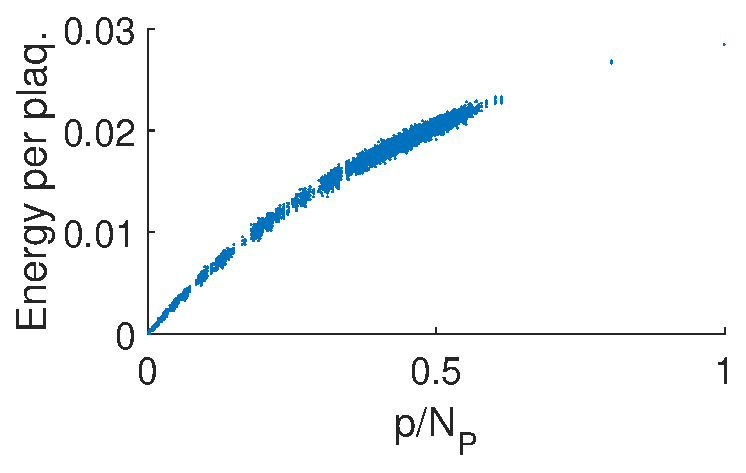
\includegraphics[width=0.4\linewidth]{stretch_En_rmax_15_b_10_s_40.eps} 
	\caption{Distribution of energy values at the flux configurations sampled. Each sector that was sampled has at least 5 points, but many are not sampled at all if their expected contribution is too low.} 
	\label{EndistPlot}
\end{figure}

\begin{figure}
	\centering
	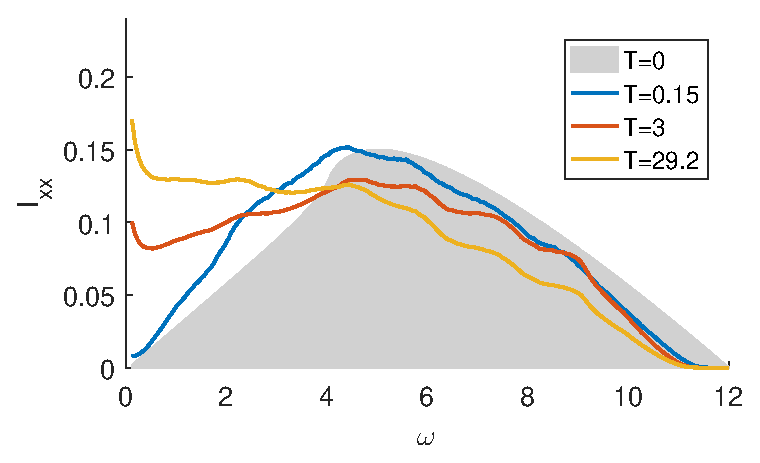
\includegraphics[width=0.43\linewidth]{stretch_Ixx_special_b_rmax_11_b_10_s_0.eps} 
	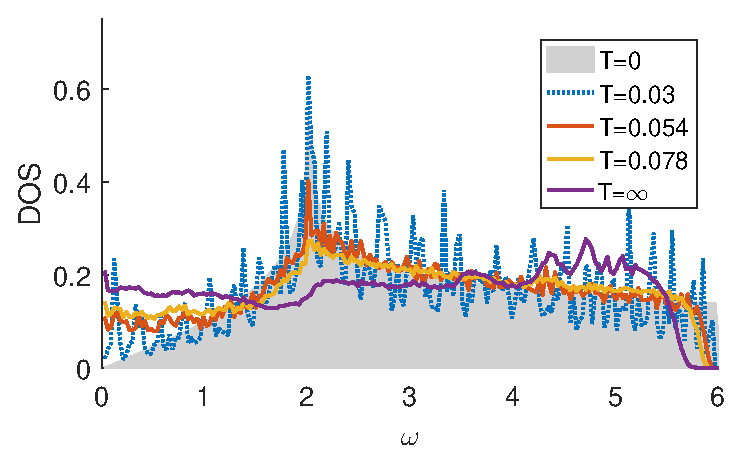
\includegraphics[width=0.43\linewidth]{stretch_DOS_special_b_rmax_7_b_10_s_0.eps} 
	\caption{Plots of unstrained Raman and DOS to compare with Ref. \cite{Nasu16} Fig. 3(a) and Ref. \cite{Nasu15} Fig. 3(a). resp. The comparisons appear quite favorable, although the present study did not involve the superlattice treatment that allowed Ref. \cite{Nasu15} to suppress the finite-size effects that are large in our plot of the DOS. The system sizes used were $ r = 11$ and $r=7$ chosen to most closely mimich the ones used in those references. }
	\label{comparePlots}
\end{figure}


	
\end{document}